\documentclass[12pt]{article}

\usepackage[utf8]{inputenc}
\usepackage[russian]{babel}
\usepackage{graphicx}
\usepackage{indentfirst}
\usepackage{booktabs}


\graphicspath{{pic/}}

\begin{document}

\begin{center}
	\LARGE 
	\textbf{Практическое занятие 5}\\
	РЕШЕНИЕ ТИПОВЫХ ЗАДАЧ АЛГЕБРЫ И АНАЛИЗА\\
\end{center}

\begin{flushright}
	\large
	Игнашов Иван\\
	Вариант 8\\
\end{flushright}

\newpage

 \section*{1. Цель работы}
Ознакомиться с возможностями системы MATLAB в решении типовых задача алгебры и анализа, изучение встроенного пакета символьных вычислений и операций Symbolic Math Toolbox.
\subsection*{Порядок работы:}
\begin{enumerate}
	\item Составить и отладить программы для нахождения корней уравнения f1(x) = 0 и f2(x) = 0 и вывести графики функции\\
		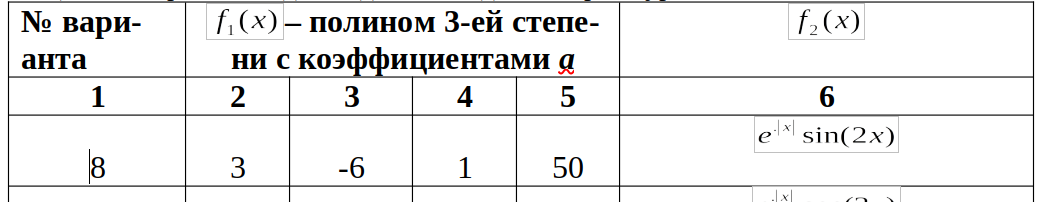
\includegraphics[width=0.75\linewidth]{formula.png}\\
		
	\item Найти определенный интеграл для подынтегральной функции\\
		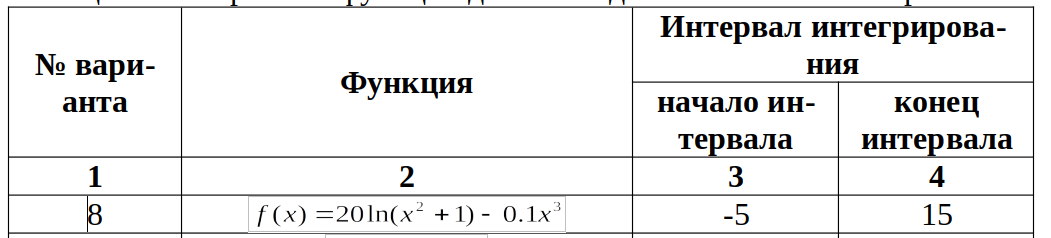
\includegraphics[width=0.4\linewidth]{formula2.png}
	\item Найти определенный интеграл для той же подынтегральной функции с использованием пакета символьных вычислений\\
\end{enumerate}

\newpage
 \section*{2. Листинг программы и результаты выполнения}%
 
 \subsection*{2.1. функции f1, f2}
\begin{figure}[!h]
	\centering
	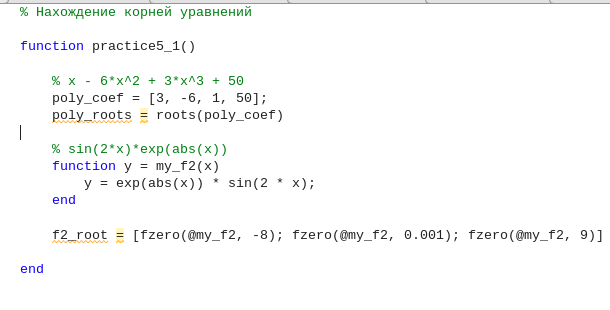
\includegraphics[width=\linewidth]{func_zeros.png}
	\caption{Программа расчёта корней для f1, f2}
\end{figure}

\begin{figure}[!h]
	\centering
	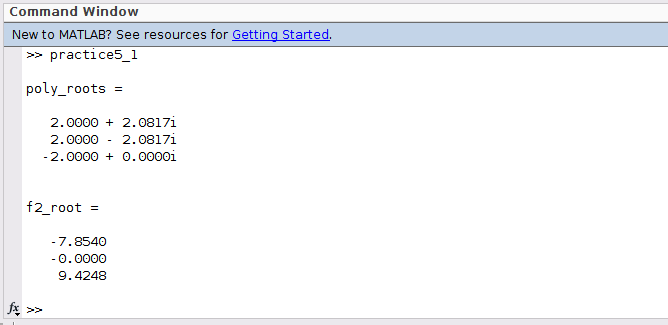
\includegraphics[width=\linewidth]{func_zeros_output.png}
	\caption{Корни функций f1, f2}
\end{figure}

\begin{figure}[!h]
	\centering
	Экран подготовки
	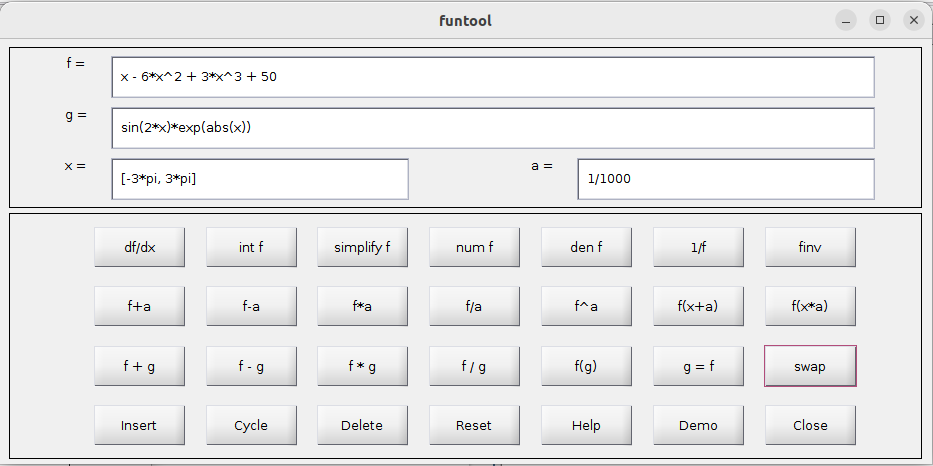
\includegraphics[width=\linewidth]{funtool_setup.png}
	Графики
	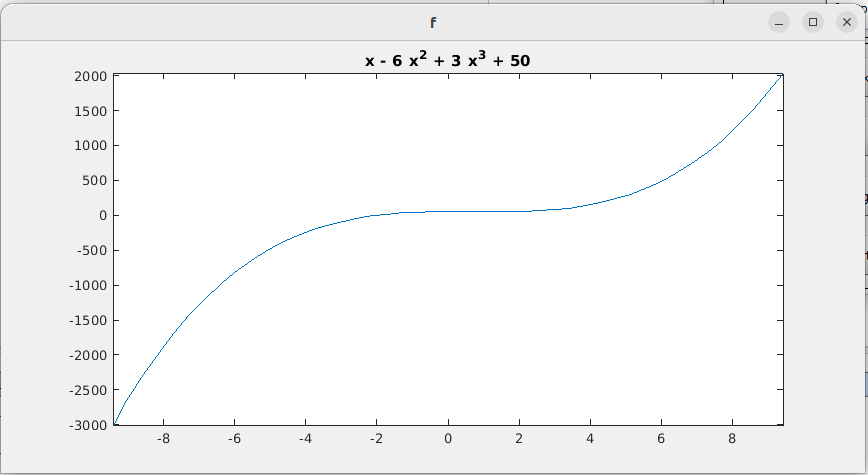
\includegraphics[width=\linewidth]{funtool_f1.png}
    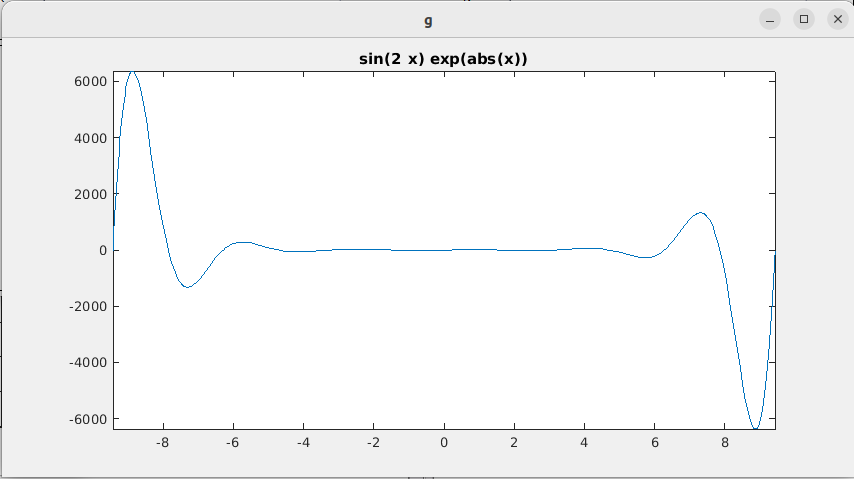
\includegraphics[width=\linewidth]{funtool_f2.png}
	\caption{Графики функций отрисованные в funtools}
\end{figure}



\begin{figure}[!h]
  \subsection*{2.2. Интегрирование f3}

	

 \end{figure}
 
 \begin{figure}[!h]
 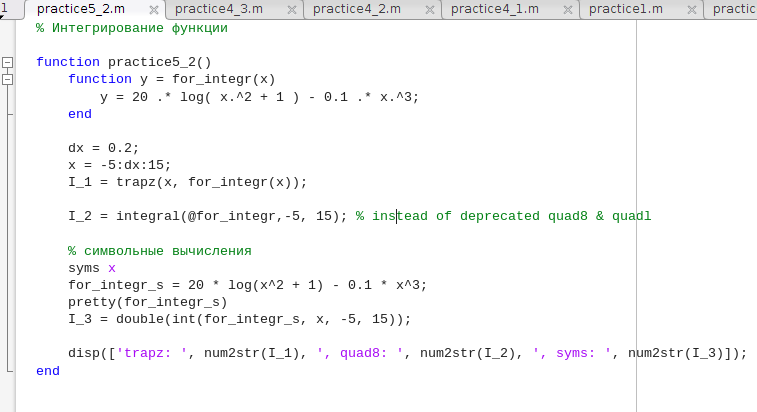
\includegraphics[width=\linewidth]{integr_setup.png}
 \caption{Листинг программы расчёта интегралов}
 \end{figure}
  int - это integrate; double - это "перевод в double", приведение к double, "решение" до 10го числа

\begin{figure}[!h]
 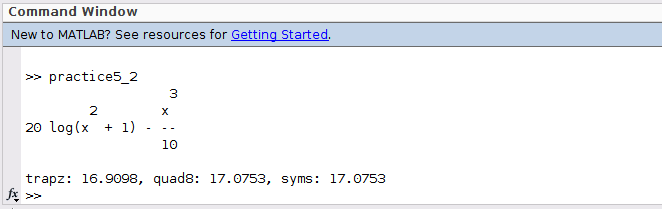
\includegraphics[width=\linewidth]{integr_output.png}
 \caption{Вывод программы}
\end{figure}
 

\end{document}